% This must be in the first 5 lines to tell arXiv to use pdfLaTeX, which is strongly recommended.
\pdfoutput=1
% In particular, the hyperref package requires pdfLaTeX in order to break URLs across lines.

\documentclass[11pt]{article}

% Remove the "review" option to generate the final version.
\usepackage{ACL2023}

% Standard package includes
\usepackage{times}
\usepackage{latexsym}

% For proper rendering and hyphenation of words containing Latin characters (including in bib files)
\usepackage[T1]{fontenc}
% For Vietnamese characters
% \usepackage[T5]{fontenc}
% See https://www.latex-project.org/help/documentation/encguide.pdf for other character sets

% This assumes your files are encoded as UTF8
\usepackage[utf8]{inputenc}

% This is not strictly necessary, and may be commented out.
% However, it will improve the layout of the manuscript,
% and will typically save some space.
\usepackage{microtype}

% This is also not strictly necessary, and may be commented out.
% However, it will improve the aesthetics of text in
% the typewriter font.
\usepackage{inconsolata}
\usepackage{multirow}

% If the title and author information does not fit in the area allocated, uncomment the following
%
%\setlength\titlebox{<dim>}
%
% and set <dim> to something 5cm or larger.

\title{News-Driven Stock Price Prediction Based on a Pretrained BERT Models}

% Author information can be set in various styles:
% For several authors from the same institution:
% \author{Author 1 \and ... \and Author n \\
%         Address line \\ ... \\ Address line}
% if the names do not fit well on one line use
%         Author 1 \\ {\bf Author 2} \\ ... \\ {\bf Author n} \\
% For authors from different institutions:
% \author{Author 1 \\ Address line \\  ... \\ Address line
%         \And  ... \And
%         Author n \\ Address line \\ ... \\ Address line}
% To start a seperate ``row'' of authors use \AND, as in
% \author{Author 1 \\ Address line \\  ... \\ Address line
%         \AND
%         Author 2 \\ Address line \\ ... \\ Address line \And
%         Author 3 \\ Address line \\ ... \\ Address line}

\author{Mingxi Liu \\
  MIDS UCB \\
  \texttt{mingxi.liu@berkeley.edu}}

\begin{document}
\maketitle
\begin{abstract}
 3-5 sentences
This document is a supplement to the general instructions for *ACL authors. It contains instructions for using the \LaTeX{} style file for ACL 2023.
The document itself conforms to its own specifications, and is, therefore, an example of what your manuscript should look like.
These instructions should be used both for papers submitted for review and for final versions of accepted papers.
\end{abstract}

% \section{Introduction}

% These instructions are for authors submitting papers to ACL 2023 using \LaTeX. They are not self-contained. All authors must follow the general instructions for *ACL proceedings,\footnote{\url{http://acl-org.github.io/ACLPUB/formatting.html}} as well as guidelines set forth in the ACL 2023 call for papers.\footnote{\url{https://2023.aclweb.org/calls/main_conference/}} This document contains additional instructions for the \LaTeX{} style files.
% The templates include the \LaTeX{} source of this document (\texttt{acl2023.tex}),
% the \LaTeX{} style file used to format it (\texttt{acl2023.sty}),
% an ACL bibliography style (\texttt{acl\_natbib.bst}),
% an example bibliography (\texttt{custom.bib}),
% and the bibliography for the ACL Anthology (\texttt{anthology.bib}).

% \section{Engines}

% To produce a PDF file, pdf\LaTeX{} is strongly recommended (over original \LaTeX{} plus dvips+ps2pdf or dvipdf). Xe\LaTeX{} also produces PDF files, and is especially suitable for text in non-Latin scripts.
% \begin{table}
% \centering
% \begin{tabular}{lc}
% \hline
% \textbf{Command} & \textbf{Output}\\
% \hline
% \verb|{\"a}| & {\"a} \\
% \verb|{\^e}| & {\^e} \\
% \verb|{\`i}| & {\`i} \\ 
% \verb|{\.I}| & {\.I} \\ 
% \verb|{\o}| & {\o} \\
% \verb|{\'u}| & {\'u}  \\ 
% \verb|{\aa}| & {\aa}  \\\hline
% \end{tabular}
% \begin{tabular}{lc}
% \hline
% \textbf{Command} & \textbf{Output}\\
% \hline
% \verb|{\c c}| & {\c c} \\ 
% \verb|{\u g}| & {\u g} \\ 
% \verb|{\l}| & {\l} \\ 
% \verb|{\~n}| & {\~n} \\ 
% \verb|{\H o}| & {\H o} \\ 
% \verb|{\v r}| & {\v r} \\ 
% \verb|{\ss}| & {\ss} \\
% \hline
% \end{tabular}
% \caption{Example commands for accented characters, to be used in, \emph{e.g.}, Bib\TeX{} entries.}
% \label{tab:accents}
% \end{table}
% \section{Preamble}
% \begin{table*}
% \centering
% \begin{tabular}{lll}
% \hline
% \textbf{Output} & \textbf{natbib command} & \textbf{Old ACL-style command}\\
% \hline
% \citep{ct1965} & \verb|\citep| & \verb|\cite| \\
% \citealp{ct1965} & \verb|\citealp| & no equivalent \\
% \citet{ct1965} & \verb|\citet| & \verb|\newcite| \\
% \citeyearpar{ct1965} & \verb|\citeyearpar| & \verb|\shortcite| \\
% \citeposs{ct1965} & \verb|\citeposs| & no equivalent \\
% \citep[FFT;][]{ct1965} &  \verb|\citep[FFT;][]| & no equivalent\\
% \hline
% \end{tabular}
% \caption{\label{citation-guide}
% Citation commands supported by the style file.
% The style is based on the natbib package and supports all natbib citation commands.
% It also supports commands defined in previous ACL style files for compatibility.
% }
% \end{table*}
% The first line of the file must be
% \begin{quote}
% \begin{verbatim}
% \documentclass[11pt]{article}
% \end{verbatim}
% \end{quote}
% To load the style file in the review version:
% \begin{quote}
% \begin{verbatim}
% \usepackage[review]{ACL2023}
% \end{verbatim}
% \end{quote}
% For the final version, omit the \verb|review| option:
% \begin{quote}
% \begin{verbatim}
% \usepackage{ACL2023}
% \end{verbatim}
% \end{quote}
% To use Times Roman, put the following in the preamble:
% \begin{quote}
% \begin{verbatim}
% \usepackage{times}
% \end{verbatim}
% \end{quote}
% (Alternatives like txfonts or newtx are also acceptable.)
% Please see the \LaTeX{} source of this document for comments on other packages that may be useful.
% Set the title and author using \verb|\title| and \verb|\author|. Within the author list, format multiple authors using \verb|\and| and \verb|\And| and \verb|\AND|; please see the \LaTeX{} source for examples.
% By default, the box containing the title and author names is set to the minimum of 5 cm. If you need more space, include the following in the preamble:
% \begin{quote}
% \begin{verbatim}
% \setlength\titlebox{<dim>}
% \end{verbatim}
% \end{quote}
% where \verb|<dim>| is replaced with a length. Do not set this length smaller than 5 cm.

\section{Introduction 1 page}

Financial news is among the forces that move the stock market. Investors have been trying to build models based on news text information to predict the movements of the stock market. Such practice usually consists of two tasks: sentiment analysis of the news and predicting the price movement based on the sentiment scores. The Transformer models have brought NLP tasks to a new level. With the help of pre-trained BERT models, sentiment analysis of financial news now can be done with higher accuracy and less challenge.

However, better sentiment analysis does not necessarily bring better stock price prediction and investment results. As shown in this paper, during the outbreak of COVID-19 in 2020, while negative sentiments were still dominating the news media, the stock market rebounded with the help of monetary easing and fiscal stimulus. As a result, models based directly on the sentiment classification results of the pre-trained models performed poorly. The models extract more information from the news (such as their importance or relevance to the stock market) besides the sentiment to make good predictions.

Luckily the BERT models provide flexibility in extracting deeper layers of information from the news, including the Pooler tokens, the Cls tokens, and other hidden states. Considering the data size, we choose to extract the Pooler tokens and build different models upon them.

We use news from Reuters to predict the daily movements of S\&P 500 Index. The total number of pieces of news is around 138,000 and the total number of price data is around 2,400. We explore several methods to aggregate the news within a day.

Although some past research treated the prediction of stock price movement as a classification problem, we argue the continuous nature of price makes it more suitable for a regression problem. The predictions of the models are converted into simulated trading signals, which enables us to evaluate the models with financial metrics such as Sharpe Ratio and Max Drawdown in addition to statistical metrics.

The result shows models based on the Pooler tokens generally outperform those directly based on the sentiment classifications. Furthermore, the nature of news-driven stock prediction is similar to sequence-to-sequence learning. Inspired by the success of transformer models, we propose a model with encoder-decoder architecture and attention mechanism. Its ability to connect information from both news and past stock price movement patterns makes it outperform other models.



\section{Background 1/2 page}

It's no news that news is used to predict stock price movements(e.g. \citealp{Tetlock:2007}). Since it's an interdisciplinary task involving NLP and financial engineering, the solution evolves with the progress on either side. On the NLP side, the essential problem is how to extract numeric information from the text of news. Early work used the bag-of-words as text representation to perform sentiment analysis for the news. For example, \citet{Schumaker:2009} examines a predictive machine learning approach for financial news article analysis using several different textual representations: bag of words, noun phrases, and named entities. Later work adopted word embeddings such as Word2Vec.\citet{Hu:2018} propose a Hybrid Attention Network to predict the stock trend based on the sequence of recent related news and employ self-paced learning for effective and efficient learning. They use a pre-trained Word2Vec embedding layer to calculate the embedded vector for each word and then average all the words' vectors to construct a news vector. Other techniques include character-based neural language model \citep{dos-santos-pinheiro-dras-2017-stock} and topic modeling \citep{nguyen-shirai-2015-topic}. Since BERT became the state-of-art NLP model, researchers have been trying to apply it to the task above(see \citet{sawhney-etal-2021-quantitative} and \citet{tsutsumi-utsuro-2022-detecting}). 

As with other applications of BERT, fine-tuning may further improve the performance. A lot of recent works have been focused on further training BERT on financial domain corpora(see \citet{araci2019finbert}) or even training BERT from scratch on financial domain corpora(see \citet{yang2020finbert} and \citet{ijcai2020p622}). \citet{peng-etal-2021-domain} points out that continual training from the original BERT model is more effective than domain-specific pretraining from scratch. This paper proposes a third option: fine-tuning with the stock price data. This can be done by retraining certain layers of BERT during the training for the prediction task. The process is similar to sentiment analysis, only the sentiment is labeled by the change in stock price.


\section{Methods 2-3 pages}

\subsection{Problem Description}

For stock prediction problems, the ultimate goal is to generate a signal $S$ which represents the ratio of stock holding value to the investor's total assets. We constrain $S \in [-1,1]$, which means short-selling is allowed but leverage is not.

Although the task can be viewed as a classification problem if we only predict whether the stock price is going up or down, however, the long-term uptrend of S\&P 500 index suggests there are more "up" days than "down" days, thus the samples are imbalanced. Some previous research tries to avoid this problem by using other thresholds instead of zero \citep{xu-cohen-2018-stock}. However, the choices of these thresholds are arbitrary and are difficult to justify. For example, if we set thresholds at 0 and 1, is it reasonable to label 0.99 and 1.01 as different classes while 0.01 and 0.99 the same class? Essentially, the returns of stocks are continuous rather than discrete, so we prefer to view it as a regression problem.

In our context, the problem is how to use the news as input to generate a continuous signal $S$, where $S \in [-1,1]$. This enables us to directly simulate the investment returns by multiplying $S$ with stock returns. Outputs or predictions from different models are first standardized into z-score and transferred with $tanh$ function to generate signal S. In this way the financial metrics from different models are comparable. The benefit of this simulated trading is that we can use investment performance metrics such as the Sharpe Ratio and Max Drawdown in addition to statistical metrics to evaluate the predictions. The Sharpe Ratio is a measure of risk-adjusted return. It compares the average return of an investment to its standard deviation. Max Drawdown is the largest peak-to-trough decline in the value of an investment or trading strategy over a specific period. Both are two key metrics used to evaluate the risk and return of an investment or trading strategy. 


\subsection{Data}

This paper experiments on predicting the daily change of S\&P 500 Index based on financial headline reports of Reuters. In order to get as many samples as possible, two sources of news data are combined together. One is from \citet{ding-etal-2014-using}, which covers the period from October 2006 to November 2013, totally 105,343 pieces. This time span witnesses a severe economic downturn in 2007-2010, followed by a modest recovery in 2011-2013. The other is provided by Kaggle, which includes 32,770 Reuters news from March 2018 to July 2020, which also covers a volatile period during Cov-19. Since both sources are from Reuters and are comparable in frequency and length, we think it's reasonable to combine them together. The gap between 2013 to 2018 is not a big issue if we use the first source as training set and the second validation/test set. 

The lead paragraph (normally the first paragraph) of each news is selected as the input. It typically contains 30~50 words, providing more complete information than the title which contains less than 10 words and requring less computing resources than the full content.

The S\&P 500 Index price data comes from Yahoo Finance. It contains a daily series covering both periods above. The log-returns of the index is used as the predicting target. The size of the labels is 2,393 after aligning the dates with the news data. 

Note that the number of news is more than 50 times of the number of labels. This is because there are usually 40 to 60 news per day. Therefore, we need to aggregate the information of news of the same day. Different methods will be discussed in the following sections. 

\subsection{Experiments}

In this section, we compare five methods of extracting and processing the information from news text. Their major differences are listed in Table \ref{tab:experiment_details}

\begin{table*}[t]
  \centering
  \begin{tabular}{|c|c|c|c|}
  \hline
  Models & NLP Model & Output from NLP model & Aggregation method \\
  \hline
  Lexicon Senti & Vader (lexicon) & Prob(P)-Prob(N) & Intraday simple average \\
  FinBERT Senti & FinBERT & Prob(P)-Prob(N) & Intraday simple average \\
  FB Avg & FinBERT & Pooler & Intraday simple average \\
  FB Attention & FinBERT & Pooler & Intraday attention\\
  FB LSTM & FinBERT & Pooler &  Intra-\&inter-day attention\\
  FB Transformer & FinBERT & Pooler &  Intra-\&inter-day attention\\
  \hline
  \end{tabular}
  \caption{Major settings of the Models}
  \label{tab:experiment_details}
\end{table*}

\textbf{Baseline: lexicon-based sentiment analysis.} We use a lexicon-based sentiment analysis similar to \citet{hao2021} as the baseline. The NLTK package provides a version of VADER \citep{Hutto_Gilbert_2014} sentiment analysis. It generates the probabilities of Positive, Negative, and Neutral. We take Prob(Positive)-Prob(Negative) and average the values within the same day as the output.

\textbf{FinBERT Senti.} FinBERT is a BERT model pre-trained on financial communication text \citep{yang2020finbert}. Previous research shows this type of pre-trained BERT models outperforms bag-of-word or rule-based models \citep{yang2020finbert,ijcai2020p622,araci2019finbert}. We convert the logits output from FinBERT to probabilities of Positive, Negative and Neutral. The rest procedures are the same with the baseline. The comparison between these two can provide some evidence that whether better sentiment analysis brings better stock price prediction. 

\textbf{FB Avg.} One advantage of the BERT models is that we can fine-tune it with our own data. Constrained by our data size and computing resources, we take the pooler output from the FinBERT model, instead of applying other deeper fine-tuning methods. The pool output of any piece of news has a shape of (768,). With truncating and padding, we take 50 pooler outputs of news per day, so the shape of input for each day is (50,768). For this FB Avg model, we simply average the 50 pooler outputs to get a daily representation with shape (1,768). Then we add a Dense(32) layer and a Dropout(0.3) layer on top of it, followed by the final Dense(1) output layer.   

\textbf{FB Attention.} This model replaces the simple average step of FB Avg with weighted average using Self-Attention mechanism. The intuition is that some news or some aspects of the news may be more related with the change of stock price than other. The rest of model settings are the same with FB Avg.

\textbf{FB Transformer.} The models above only use the information within a day. We can further extend the model to include the information from the historical news. For instance, a neutral sentiment after several positive sentiment may indicate things are getting worse, while a neutral sentiment after several negative sentiment may indicate things a getting better, and they may have different implications for stock price movements. Once we include the historical information, our task becomes a sequence-to-sequence task. Inspired by the success of transformers in sequence-to-sequence task tasks, we build a mini-transformer for our task.

The architecture of our mini-transformer model is shown in Figure \ref{fig:fb_transformer}. Similar to \citet{NIPS2017_3f5ee243}, we have two inputs: tokenized text data and lagged outputs. Both inputs contain information for the past 60 days. For example, on day T, we use both the news and the historical returns of S\&P 500 Index from day T-59 to day T as input to predict return on day T+1. Then we roll them for 1 day to predict returns on day T+2 and so on. The text input has a shape of (60,50,768), with the first dimension indicating the number of days, the second the number of news per day and the third the token dimension. The historical return input has a shape of (60,). We also add a Multi-head Attention layer to each of the text and return input. Then we use a Cross Attention layer to connect the two inputs and feed the output to three Dense layers to generate the final output.

Major differences between our mini transformer with the original one include: 1) due to limited data size, we only have 1 attention layer each instead of 6. As a result, the residual connection (Add\&Norm) is not needed. 2) Instead of adding positional encodings to the inputs, we include the positional index as a seperate feature. The reason is that, unlike \citet{NIPS2017_3f5ee243}, which is trained from scratch, our model is based on a pretrained model and we don't have enough data to perform a deep fine-tuning. Simply adding positional encodings to the tokens will distort the pretrained tokens. Since the length of sequence is fixed at 60, we can use a integer sequence from 1 to 60 each divided by 60 as the positional index. 3) The original transformer use a causal attention in the decoder to prevent the use of future data. Since we already prevent the use of future data with a rolling window, our model uses a global attention.

\textbf{FB LSTM.} "RNN+Attention" was the state-of-art architecture to build seq2seq models before Transformers. We also build an LSTM+Attention model to compare with the mini transformer model. The architecture is shown in Figure \ref{fig:fb_lstm}. It has the same inputs structure with FB Transformer and the use of attention mechanism is similar. Since the LSTM handles the sequence order, the positional encodings are no longer needed.

\subsection{Model Training}

We use KerasTuner\footnote{\url{https://keras.io/keras_tuner/}} to tune hyperparameters including model parameters such as the number of attention heads and training settings such as learning rate. The details are given in Appendix. KerasTuner helps select the best-performing hyperparameters based on validation MSE. We further train the models, select the best ones based on validation MSE, and generate the evaluation results on the test set.

\section{Result and discussion 1 - 2 pages}

  \begin{table*}
  \centering
  \begin{tabular}{c|cccc|ccc}
     & \multicolumn{4}{|c|}{Statistical Metrics} & \multicolumn{3}{c}{Financial Metrics} \\
    \multirow{2}{2em}{Models} & \multirow{2}{2em}{Pearson Corr.} & \multirow{2}{2em}{Spearman Corr.} & \multirow{2}{*}{MAE} & \multirow{2}{*}{MSE} & \multirow{2}{2em}{Total Return} & \multirow{2}{2em}{Sharpe Ratio} & \multirow{2}{2em}{Max Drawdown} \\
    & & & & & & & \\
    \hline
    Target & 100.00\% & 100.00\% & n.a. & n.a. & 13.53\% & 0.36 & -41.44\% \\
    Lexicon Senti & 2.24\% & -0.26\% & n.a. & n.a. & 8.98\% & 0.33 & -20.18\% \\
    FinBERT Senti & -1.29\% & -2.91\% & n.a. & n.a. & 2.63\% & 0.09 & -22.94\% \\
    FB Avg & 1.22\% & 1.29\% & 0.0867 & 0.0089 & 2.63\% & 0.10 & -27.11\% \\
    FB Attention & 4.13\% & 4.35\% & 0.0150 & 0.0005 & 14.15\% & 1.21 & -9.27\% \\
    FB LSTM & 14.24\% & 6.49\% & 0.0882 & 0.0135 & 41.44\% & 1.57 & -12.32\% \\
    FB Transformer & 13.01\% & 12.60\% & 0.0170 & 0.0005 & 58.27\% & 2.15 & -6.17\% \\

    \end{tabular}
    \label{tab:results}
    \caption{Table caption goes here.}
  \end{table*}

The statistical and financial metrics of the models are shown in Table \ref{tab:results}. Key observations from the results are:

\begin{enumerate}
  \item FB Transformer performs the best from both statistical and financial perspective. It has the highest correlation with the target and lowest predicting errors. It also brings the highest return in absolute terms as well as in risk-adjusted measures.
  \item The two models with encoder-decoder architecture (FB Transformer, FB LSTM) outperform other models, suggesting the inclusion of historical news and stock price changes help improve the predictive power of the model.
  \item FB Attention outperforms FB Avg, suggesting replacing simple average with Self-Attention based weighted average improves the model.
  \item Finally, models based on the final sentiment classifications (Lexicon Senti and FinBERT Senti) underperform those based on Pooler tokens, suggesting the sentiment alone does not provide enough information for predicting the stock movements. FinBERT Senti even underperforms Lexicon Senti, an evidence that better sentiment analysis does not guarantee better stock price prediction.
\end{enumerate}


\begin{figure}[h!]
  \centering
  \begin{subfigure}[b]{0.4\textwidth}
    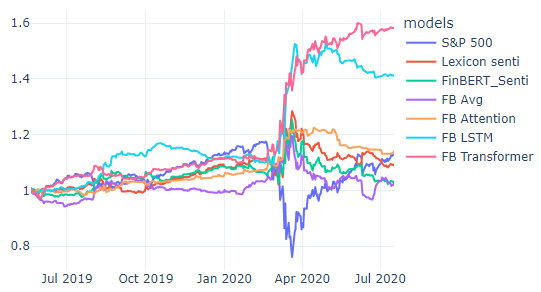
\includegraphics[width=\textwidth]{total_returns.png}
    \caption{Simulated total wealth of \$1 investment based on different model signals}
    \label{fig:total_return}
  \end{subfigure}
  \begin{subfigure}[b]{0.4\textwidth}
    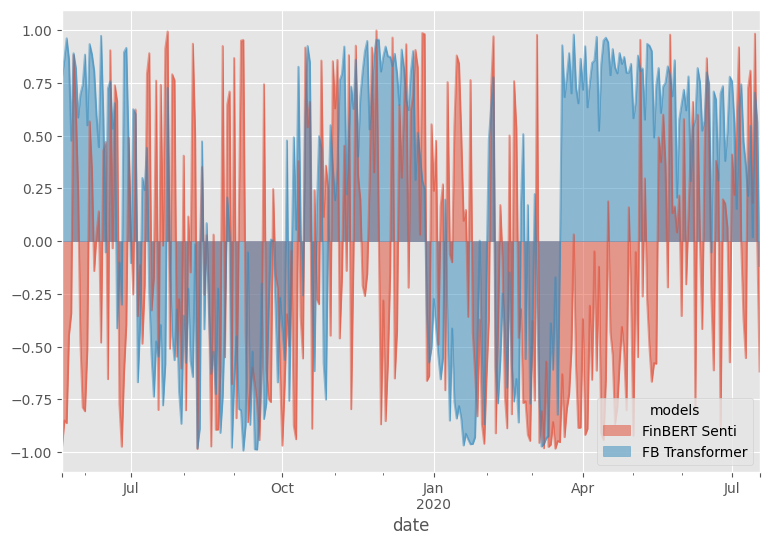
\includegraphics[width=\textwidth]{signal_compare.png}
    \caption{Signals of FB Transformer adjusted much faster than FinBERT Senti in Mar 2020}
    \label{fig:signal_compare}
  \end{subfigure}
\end{figure}

Figure \ref{fig:total_return} provides a more intuitive illustration of the performance of the models. It shows if we invested 1 dollar based on the signals of different models at the begin of the test period, how much it would become over time. The figure shows the major divergence among different models happened during the period from March 2020 to Jun 2020. During this time, S\&P 500 Index rebounded strongly with the help of unprecedented monetary easing and fiscal stimulus, but the number of new cases in US increased to 10,000 per day, which naturally dragged the overall sentiment in financial media. 



1) a lexicon-based sentiment analysis; 2) sentiment analysis output by FinBert a BERT model pre-trained on financial contents; 3) predicting based on pooler output of FinBert model; 4) predicting based on pooler output of FinBert model with attention mechanism; 5) predict based on pooler output 

Each tweet is embedded with one of the BERT variants above. The output vector for the [CLS] token goes to the next step (subject to change).

\subsection{Daily aggregation}
Since there may be more than one tweet for a stock in a day, the information from these tweets must be aggregated to generate one signal. RNN, attention-based weighted average, or simple average may be used for the aggregation, depending on time and computing resources. 

\subsection{Prediction}
The final layer of the model is a Softmax layer predicting the next day's price movement in three direction categories: up, down, or flat(within a certain range). Metrics such as loss and accuracy can be compared at this step.

\subsection{Trading simulation}
According to the prediction from the model, we can decide to buy, sell, or do nothing with the targeted stock. Then we can calculate this simulated investment return and evaluate its investing performance with financial metrics such as the Sharpe Ratio, which are more important than loss or accuracy for investment.

\subsection{Customized loss function (Optional)}
The last two steps can be combined together using a customized loss function which is directly related to the investment performance. Models trained under this customized loss function may generate better investment results.

\section{Result and discussion 1 - 2 pages}

\section{Conclusion 3-5 sentences}

% See Table~\ref{tab:accents} for an example of a table and its caption.
% \textbf{Do not override the default caption sizes.}

% \subsection{Hyperlinks}

% Users of older versions of \LaTeX{} may encounter the following error during compilation: 
% \begin{quote}
% \tt\verb|\pdfendlink| ended up in different nesting level than \verb|\pdfstartlink|.
% \end{quote}
% This happens when pdf\LaTeX{} is used and a citation splits across a page boundary. The best way to fix this is to upgrade \LaTeX{} to 2018-12-01 or later.

% \subsection{Citations}

% What do you plan to do?
% Why is it important, and why is it challenging?
% What dataset(s) will you use?
% What algorithms might you use? Are good implementations available, or will you need to write your own? (Don’t worry if you can’t answer this well at this stage of the course.)
% References to at least four papers related to your proposal

% Table~\ref{citation-guide} shows the syntax supported by the style files.
% We encourage you to use the natbib styles.
% You can use the command \verb|\citet| (cite in text) to get ``author (year)'' citations, like this citation to a paper by \citet{Gusfield:97}.
% You can use the command \verb|\citep| (cite in parentheses) to get ``(author, year)'' citations \citep{Gusfield:97}.
% You can use the command \verb|\citealp| (alternative cite without parentheses) to get ``author, year'' citations, which is useful for using citations within parentheses (e.g. \citealp{Gusfield:97}).

% \subsection{References}

% \nocite{Ando2005,augenstein-etal-2016-stance,andrew2007scalable,rasooli-tetrault-2015,goodman-etal-2016-noise,harper-2014-learning}

% The \LaTeX{} and Bib\TeX{} style files provided roughly follow the American Psychological Association format.
% If your own bib file is named \texttt{custom.bib}, then placing the following before any appendices in your \LaTeX{} file will generate the references section for you:
% \begin{quote}
% \begin{verbatim}
% \bibliographystyle{acl_natbib}
% \bibliography{custom}
% \end{verbatim}
% \end{quote}
% You can obtain the complete ACL Anthology as a Bib\TeX{} file from \url{https://aclweb.org/anthology/anthology.bib.gz}.
% To include both the Anthology and your own .bib file, use the following instead of the above.
% \begin{quote}
% \begin{verbatim}
% \bibliographystyle{acl_natbib}
% \bibliography{anthology,custom}
% \end{verbatim}
% \end{quote}
% Please see Section~\ref{sec:bibtex} for information on preparing Bib\TeX{} files.

% \subsection{Appendices}

% Use \verb|\appendix| before any appendix section to switch the section numbering over to letters. See Appendix~\ref{sec:appendix} for an example.

% \section{Bib\TeX{} Files}
% \label{sec:bibtex}

% Unicode cannot be used in Bib\TeX{} entries, and some ways of typing special characters can disrupt Bib\TeX's alphabetization. The recommended way of typing special characters is shown in Table~\ref{tab:accents}.

% Please ensure that Bib\TeX{} records contain DOIs or URLs when possible, and for all the ACL materials that you reference.
% Use the \verb|doi| field for DOIs and the \verb|url| field for URLs.
% If a Bib\TeX{} entry has a URL or DOI field, the paper title in the references section will appear as a hyperlink to the paper, using the hyperref \LaTeX{} package.

% \section*{Limitations}
% ACL 2023 requires all submissions to have a section titled ``Limitations'', for discussing the limitations of the paper as a complement to the discussion of strengths in the main text. This section should occur after the conclusion, but before the references. It will not count towards the page limit.
% The discussion of limitations is mandatory. Papers without a limitation section will be desk-rejected without review.

% While we are open to different types of limitations, just mentioning that a set of results have been shown for English only probably does not reflect what we expect. 
% Mentioning that the method works mostly for languages with limited morphology, like English, is a much better alternative.
% In addition, limitations such as low scalability to long text, the requirement of large GPU resources, or other things that inspire crucial further investigation are welcome.

% \section*{Ethics Statement}
% Scientific work published at ACL 2023 must comply with the ACL Ethics Policy.\footnote{\url{https://www.aclweb.org/portal/content/acl-code-ethics}} We encourage all authors to include an explicit ethics statement on the broader impact of the work, or other ethical considerations after the conclusion but before the references. The ethics statement will not count toward the page limit (8 pages for long, 4 pages for short papers).

% \section*{Acknowledgements}
% This document has been adapted by Jordan Boyd-Graber, Naoaki Okazaki, Anna Rogers from the style files used for earlier ACL, EMNLP and NAACL proceedings, including those for
% EACL 2023 by Isabelle Augenstein and Andreas Vlachos,
% EMNLP 2022 by Yue Zhang, Ryan Cotterell and Lea Frermann,
% ACL 2020 by Steven Bethard, Ryan Cotterell and Rui Yan,
% ACL 2019 by Douwe Kiela and Ivan Vuli\'{c},
% NAACL 2019 by Stephanie Lukin and Alla Roskovskaya, 
% ACL 2018 by Shay Cohen, Kevin Gimpel, and Wei Lu, 
% NAACL 2018 by Margaret Mitchell and Stephanie Lukin,
% Bib\TeX{} suggestions for (NA)ACL 2017/2018 from Jason Eisner,
% ACL 2017 by Dan Gildea and Min-Yen Kan, NAACL 2017 by Margaret Mitchell, 
% ACL 2012 by Maggie Li and Michael White, 
% ACL 2010 by Jing-Shin Chang and Philipp Koehn, 
% ACL 2008 by Johanna D. Moore, Simone Teufel, James Allan, and Sadaoki Furui, 
% ACL 2005 by Hwee Tou Ng and Kemal Oflazer, 
% ACL 2002 by Eugene Charniak and Dekang Lin, 
% and earlier ACL and EACL formats written by several people, including
% John Chen, Henry S. Thompson and Donald Walker.
% Additional elements were taken from the formatting instructions of the \emph{International Joint Conference on Artificial Intelligence} and the \emph{Conference on Computer Vision and Pattern Recognition}.

% Entries for the entire Anthology, followed by custom entries
\bibliography{anthology,custom}
\bibliographystyle{acl_natbib}

\appendix

\section{Appendix}

\begin{figure}[h]
  \centering
  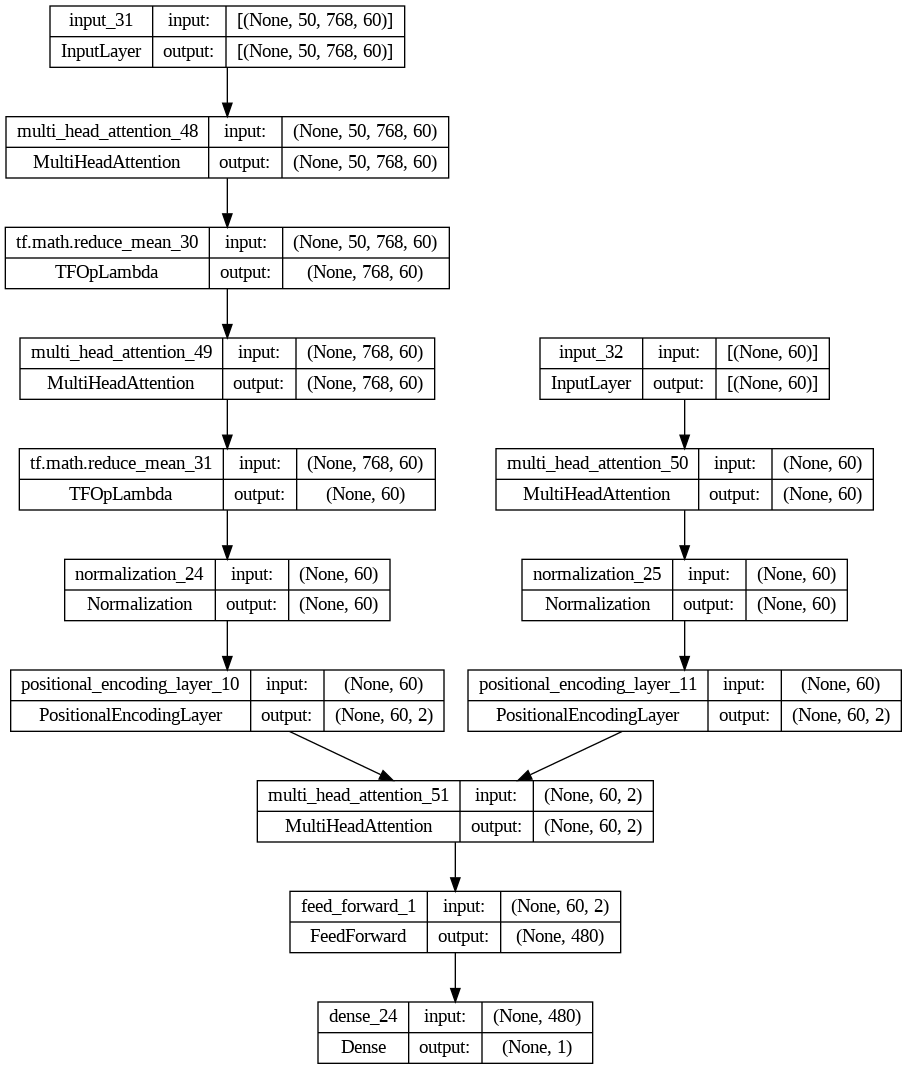
\includegraphics[width=\textwidth]{transformer_structure.png}
  \caption{The architecture of FB Transformer}
  \label{fig:fb_transformer}
\end{figure}

\begin{figure}[h]
  \centering
  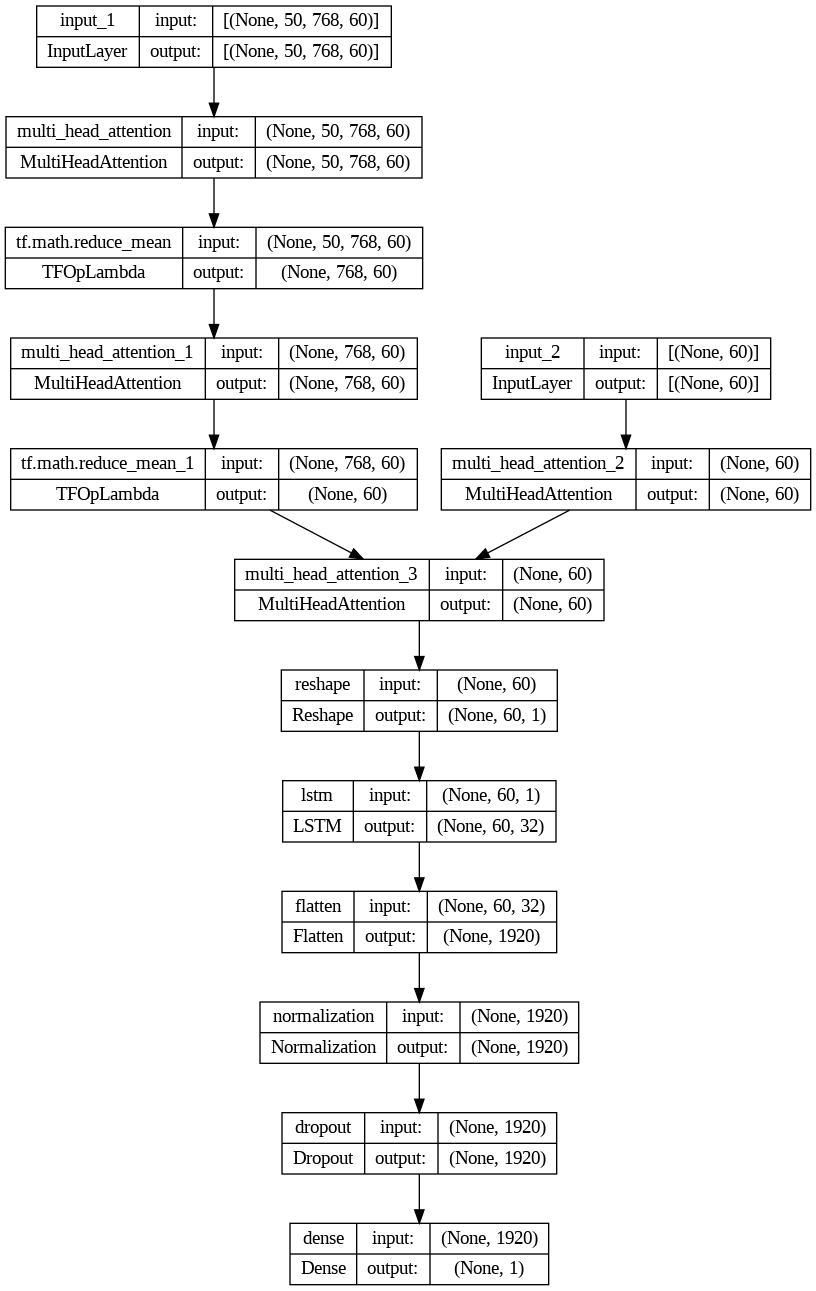
\includegraphics[width=\textwidth]{lstm.png}
  \caption{The architecture of FB LSTM}
  \label{fig:fb_lstm}
\end{figure}

\begin{figure}[h]
  \centering
  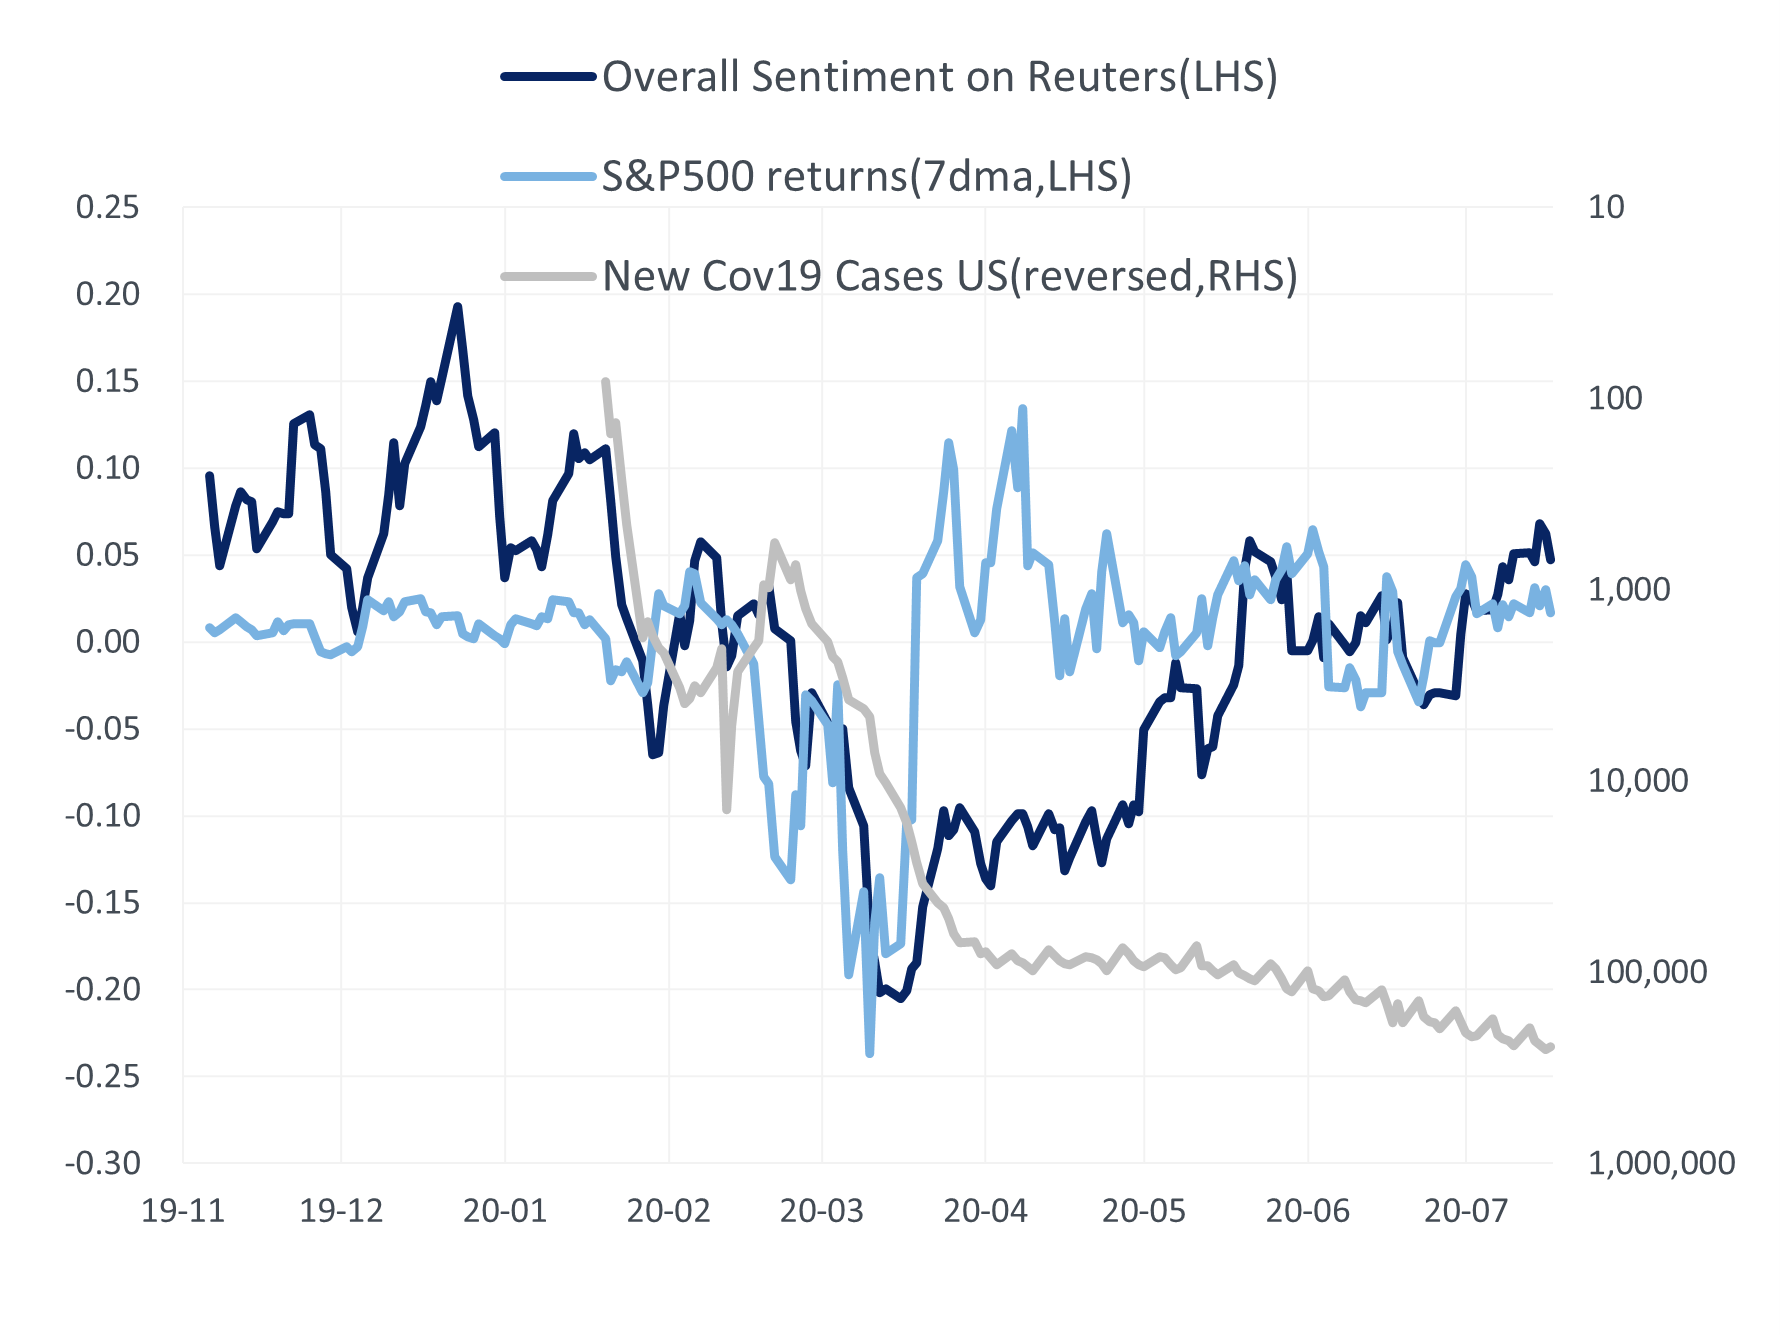
\includegraphics[width=\textwidth]{cov_vs_senti.png}
  \caption{The overall sentiment was dragged by new Cov-19 case numbers while the stock market rebounded strongly during March 2020}
  \label{fig:cov_vs_senti}
\end{figure}

% This is a section in the appendix.

\end{document}
